
% This LaTeX was auto-generated from MATLAB code.
% To make changes, update the MATLAB code and republish this document.

\documentclass{article}
\usepackage{graphicx}
\usepackage{color}

\sloppy
\definecolor{lightgray}{gray}{0.5}
\setlength{\parindent}{0pt}

\begin{document}

    
    
\section*{Zachary Kaplan}

\begin{par}
Math 440 Computational Lab \#1 2/19/19
\end{par} \vspace{1em}
\begin{par}
An online version of this file published to latex can be found at: https://www.overleaf.com/read/zvtjspxrnqkv
\end{par} \vspace{1em}
\begin{par}
\textbf{NOTE}: To render latex from this document locally, please include the         following package dependencies:
\end{par} \vspace{1em}

\begin{verbatim}\usepackage[margin=1in]{geometry}
\usepackage{amsmath}
\usepackage{amssymb}
\usepackage{microtype}
\usepackage{csquotes}\end{verbatim}
    
\subsection*{Contents}

\begin{itemize}
\setlength{\itemsep}{-1ex}
   \item The Model and Discretization
   \item Upwinding
   \item Declaration of Constants
   \item Validation of Implementation
   \item Linear Solution
   \item Quadratic Solution
   \item Sinusoidal Solution
   \item Results - Diffusion Only
   \item Results - Diffusion \& Convection
   \item Implementation of ODE solver
\end{itemize}


\subsection*{The Model and Discretization}

\begin{par}
Consider the differential operator
\end{par} \vspace{1em}
\begin{par}
$$ D_T[\cdot] = -\frac{d}{dz}\left(\kappa \frac{d}{dz}\right)
                +\nu\rho C \frac{d}{dz}
              = -\kappa \frac{d^2}{dz^2} + \nu\rho C \frac{d}{dz}, $$
\end{par} \vspace{1em}
\begin{par}
and the driving function
\end{par} \vspace{1em}
\begin{par}
$$ Q(z) = \begin{cases}
            0 & 0 \le z \le a \\
            Q_0 \cdot \sin\left(\frac{z - a}{b - a}\pi\right)
               & a \le z \le b \\
            0 & b \le z \le L
          \end{cases} \quad \forall z \in [0,L], $$
\end{par} \vspace{1em}
\begin{par}
where $0 \le a \le b \le L$.
\end{par} \vspace{1em}
\begin{par}
We then define the function $T(z)$ as the solution to the below system of a second order differential equation and BCs
\end{par} \vspace{1em}
\begin{par}
$$ \begin{cases}
     D_T[T(z)] = Q(z),\quad \forall z \in [0,L] \\
     T(0) = T_0 \\
     -\kappa \frac{d}{dz} T(L) = k(T(L) - T_{out})
   \end{cases}. $$
\end{par} \vspace{1em}
\begin{par}
In order to solve this system numerically, we'll first discretize the linear differential operator $D_T$ using a fixed width partition of $[0,L]$. Our fixed partition $\mathbf{Z} = \begin{pmatrix}    z_0 = 0 & z_1 = h & \ldots &  z_{N-1} = L-h & z_N = L    & z_{N+1} = L + h  \end{pmatrix}^\top $ has $N$ interior points and a grid spacing of $h = L/N$. Note that the final point $z_{N+1}$ is a $\text{\enquote{ghost point}}$ and is only introduced in order to achieve a second-order approximation of the boundary condition at the right endpoint. We let $\mathbf{Z}^0 =   \begin{pmatrix} z_1 & z_2 & \ldots & z_N \end{pmatrix}^\top$ denote the $N$ interior points of $\mathbf{Z}$. We will define our discretized approximation of $T(z)$ on $\mathbf{Z}$ as the vector $\mathbf{T} = \begin{pmatrix}    t_0 \approx T(z_0) & t_1 \approx T(z_1) & \ldots      & t_N \approx T(z_N) & t_{N+1} \approx T(z_{N+1})  \end{pmatrix}^\top $. Using the centered 3-point stencil for second derivatives, and the cenetered difference stencil for first order dirivatives, it follows trivially that $D_T$ may discretize as
\end{par} \vspace{1em}
\begin{par}
$$ D_T[T] \sim \left[
     -\frac{\kappa}{h^2} \begin{pmatrix}
        1 & -2 &  1 &  0 & 0 & \ldots &  0 \\
        0 &  1 & -2 &  1 & 0 & \ldots &  0 \\
        \vdots &  & \ddots & \ddots & \ddots &  & \vdots \\
        0 & \ldots & 0 &  1 & -2 &  1 &  0 \\
        0 & \ldots & 0 &  0 &  1 & -2 &  1 \end{pmatrix}
     +\frac{\nu\rho C}{2h} \begin{pmatrix}
        -1 &  0 & 1 &  0 & 0 & \ldots &  0 \\
        0 &  -1 &  0 & 1 & 0 & \ldots &  0 \\
        \vdots &  & \ddots & \ddots & \ddots &  & \vdots \\
        0 & \ldots & 0 &  -1 &  0 & 1 &  0 \\
        0 & \ldots & 0 &  0 &  -1 &  0 & 1 \end{pmatrix}
     \right] \mathbf{T}. $$
\end{par} \vspace{1em}
\begin{par}
The above approximates the evaluation of $D_T$ on the interior values of the discrete function $\mathbf{T}$, which we denote as $\mathbf{T}^0 =   \begin{pmatrix}t_1 & t_2 & \ldots & t_N\end{pmatrix}^\top$. Therefore, the constraints imposed by the ODE $D_T[T] = Q$ can be enforced by setting the above equal to $\begin{pmatrix}Q(z_1) & Q(z_2) & \ldots & Q(z_N)\end{pmatrix}^\top$.
\end{par} \vspace{1em}
\begin{par}
The first boundary condition can be trivially enforced by setting $t_0 = T_0$. The second boundary condition can be discretized using the centered first-order finite difference to
\end{par} \vspace{1em}
\begin{par}
$$ \begin{split}
     &-\kappa \frac{t_{N+1} - t_{N-1}}{2h} = k(t_N - T_{out}) \\
     \implies& t_N + \kappa\frac{t_{N+1} - t_{N-1}}{2kh} = T_{out}.
   \end{split} $$
\end{par} \vspace{1em}
\begin{par}
Combining all of the above into a single matrix system, we get a system of the form $A\mathbf{T} = \mathbf{b}$ where
\end{par} \vspace{1em}
\begin{par}
$$ \begin{split}
A &=
     -\frac{\kappa}{h^2} \begin{pmatrix}
        0 &  0 &  0 &  0 & 0 & \ldots &  0 \\
        1 & -2 &  1 &  0 & 0 & \ldots &  0 \\
        0 &  1 & -2 &  1 & 0 & \ldots &  0 \\
        \vdots &  & \ddots & \ddots & \ddots &  & \vdots \\
        0 & \ldots & 0 &  1 & -2 &  1 &  0 \\
        0 & \ldots & 0 &  0 &  1 & -2 &  1 \\
        0 &  0 &  0 &  0 & 0 & \ldots &  0 \end{pmatrix}
     +\frac{\nu\rho C}{2h} \begin{pmatrix}
        0 &  0 &  0 &  0 & 0 & \ldots &  0 \\
        -1 &  0 & 1 &  0 & 0 & \ldots &  0 \\
        0 &  -1 &  0 & 1 & 0 & \ldots &  0 \\
        \vdots &  & \ddots & \ddots & \ddots &  & \vdots \\
        0 & \ldots & 0 &  -1 &  0 & 1 &  0 \\
        0 & \ldots & 0 &  0 &  -1 &  0 & 1 \\
        0 &  0 &  0 &  0 & 0 & \ldots &  0 \end{pmatrix}
     +\begin{pmatrix}
        1 & 0 & 0 & \ldots & 0 \\
        0 & 0 & 0 &\ldots & 0 \\
        0 & 0 & 0 &\ldots & 0 \\
        \vdots & \ddots & \ddots & \vdots \\
        0 & \ldots & 0 & 0 & 0 \\
        0 & \ldots & 0 & 0 & 0 \\
        0 & \ldots & -\frac{\kappa}{2kh} & 1 & \frac{\kappa}{2kh}
      \end{pmatrix}, \\
\mathbf{b} &=
     \begin{pmatrix}
        T_0 & Q(z_1) & Q(z_2) & \ldots & Q(z_N) & T_{out}
     \end{pmatrix}^\top.
\end{split} $$
\end{par} \vspace{1em}
\begin{par}
By substituting $t_0 = T_0$ we can easily eliminate the first row of the above matrices. Similarly by writing the second boundary condition as
\end{par} \vspace{1em}
\begin{par}
$$ t_{N+1} = \frac{2kh}{\kappa} (T_{out} - t_N) + t_{N-1} $$
\end{par} \vspace{1em}
\begin{par}
and substituting this into the equation represented by the second to last row of A
\end{par} \vspace{1em}
\begin{par}
$$ \begin{gathered}
-\left(\frac{\nu\rho C}{2h} + \frac{\kappa}{h^2}\right) t_{N-1}
  + 2\frac{\kappa}{h^2} t_N
  + \left(\frac{\nu\rho C}{2h} - \frac{\kappa}{h^2}\right) t_{N+1}
  = Q(z_N) \\
\implies -\left(\frac{\nu\rho C}{2h} + \frac{\kappa}{h^2}\right) t_{N-1}
  + 2\frac{\kappa}{h^2} t_N
  + \left(\frac{\nu\rho C}{2h} - \frac{\kappa}{h^2}\right)
     \left(\frac{2kh}{\kappa} (T_{out} - t_N) + t_{N-1}\right)
  = Q(z_N) \\
\implies
  -2\frac{\kappa}{h^2} t_{N-1}
  + \left(2\frac{\kappa}{h^2} + K\right) t_N
  = Q(z_N) + K T_{out} \\
\mathrm{where} \quad K =
 \frac{2kh}{\kappa}\left(\frac{\kappa}{h^2} - \frac{\nu\rho C}{2h}\right)
 = \frac{2k}{h} - \frac{k\nu\rho C}{\kappa}
\end{gathered} $$
\end{par} \vspace{1em}
\begin{par}
we can eliminate the final row as well. This results in the simplified system $A^*\mathbf{T}^0 = \mathbf{b}^*$ where
\end{par} \vspace{1em}
\begin{par}
$$ \begin{split}
A^* &=
     -\frac{\kappa}{h^2} \begin{pmatrix}
        -2 &  1 &  0 & \ldots &  0 \\
         1 & -2 &  1 & \ldots &  0 \\
        \vdots & \ddots & \ddots & \ddots & \vdots \\
        0 & \ldots & 1 & -2 &  1 \\
        0 & \ldots & 0 &  1 & -2 \end{pmatrix}
     +\frac{\nu\rho C}{2h} \begin{pmatrix}
        0  &  1 &  0 & \ldots &  0 \\
        -1 &  0 &  1 & \ldots &  0 \\
        \vdots & \ddots & \ddots & \ddots & \vdots \\
        0 & \ldots &  -1 &   0 &  1 \\
        0 & \ldots &   0 &  -1 &  0 \end{pmatrix}
     +\begin{pmatrix}
        0 & 0 & \ldots & 0 \\
        0 & 0 & \ldots & 0 \\
        \vdots & \ddots & \ddots & \vdots \\
        0 & \ldots & 0 & 0 \\
        0 & \ldots & -\frac{\kappa}{h^2} + \frac{\nu\rho C}{2h} & K \\
      \end{pmatrix}, \\
\mathbf{b}^* &=
     \begin{pmatrix}
        Q(z_1)
          + T_0\left(\frac{\kappa}{h^2} + \frac{\nu\rho C}{2h} \right) &
        Q(z_2) & \ldots & Q(z_{N-1}) &
        Q(z_N) + K T_{out}
     \end{pmatrix}^\top.
\end{split} $$
\end{par} \vspace{1em}
\begin{par}
Therefore, in the lab below we will construct sparse matrix $A^*$ and vector $\mathbf{b}^*$ and numerically solve for $\mathbf{T}^0$. Then we will augment $\mathbf{T}^0$ by prepending $T_0$ to achieve the desired numerical solution.
\end{par} \vspace{1em}


\subsection*{Upwinding}

\begin{par}
In order to handle spurious osciallations that ocurred with large $\nu$, we consider replacing our first-order stencil with a backward difference. In this model, we will also remove our ghost point since we will be first order anyway.
\end{par} \vspace{1em}
\begin{par}
Our right boundary condition can be written as
\end{par} \vspace{1em}
\begin{par}
$$
  -\kappa \frac{t_N - t_{N-1}}{h} = k(t_N - T_{out})
  \implies t_N = \frac{\kappa t_{N-1} + kh T_{out}}{\kappa + kh}
$$
\end{par} \vspace{1em}
\begin{par}
leading to the following substitution in the final internal equation
\end{par} \vspace{1em}
\begin{par}
$$ \begin{gathered}
  -\left(\frac{\kappa}{h^2} + \frac{\nu\rho C}{h}\right) t_{N-2}
  + \left(2\frac{\kappa}{h^2} + \frac{\nu\rho C}{h}\right) t_{N-1}
  -\frac{\kappa}{h^2} t_N = Q(z_{N-1}) \\
  \implies
  -\left(\frac{\kappa}{h^2} + \frac{\nu\rho C}{h}\right) t_{N-2}
  + \left(2\frac{\kappa}{h^2} + \frac{\nu\rho C}{h}\right) t_{N-1}
  -\frac{\kappa}{h^2} \left(
      \frac{\kappa t_{N-1} + kh T_{out}}{\kappa + kh} \right)
  = Q(z_{N-1}) \\
  \implies
  -\left(\frac{\kappa}{h^2} + \frac{\nu\rho C}{h}\right) t_{N-2}
  + \left(2\frac{\kappa}{h^2} + \frac{\nu\rho C}{h}
      - K_{up} \kappa}\right) t_{N-1}
  = Q(z_{N-1}) + K_{up} kh T_{out}} \\
  \mathrm{where} \quad K_{up} = \frac{\kappa}{h^2(\kappa + kh)}
\end{gathered} $$
\end{par} \vspace{1em}
\begin{par}
Therefore, our new matrix system $A_{up} \mathbf{T} = \mathbf{b}_{up}$ becomes
\end{par} \vspace{1em}
\begin{par}
$$ \begin{split}
A_{up} &=
     -\frac{\kappa}{h^2} \begin{pmatrix}
        -2 &  1 &  0 & \ldots &  0 \\
         1 & -2 &  1 & \ldots &  0 \\
        \vdots & \ddots & \ddots & \ddots & \vdots \\
        0 & \ldots & 1 & -2 &  1 \\
        0 & \ldots & 0 &  1 & -2 \end{pmatrix}
     +\frac{\nu\rho C}{h} \begin{pmatrix}
         1 &  0 &  0 & \ldots &  0 \\
        -1 &  1 &  0 & \ldots &  0 \\
        \vdots & \ddots & \ddots & \vdots & \vdots \\
        0 & \ldots &  -1 &   1 &  0 \\
        0 & \ldots &   0 &  -1 &  1 \end{pmatrix}
     +\begin{pmatrix}
        0 & 0 & \ldots & 0 \\
        0 & 0 & \ldots & 0 \\
        \vdots & \ddots & \ddots & \vdots \\
        0 & \ldots & 0 & 0 \\
        0 & \ldots & 0 & -K_{up}\kappa \\
      \end{pmatrix}, \\
\mathbf{b}_{up} &=
     \begin{pmatrix}
        Q(z_1)
          + T_0\left(\frac{\kappa}{h^2} + \frac{\nu\rho C}{h} \right) &
        Q(z_2) & \ldots & Q(z_{N-2}) &
        Q(z_{N-1}) + K_{up} kh T_{out}
     \end{pmatrix}^\top.
\end{split} $$
\end{par} \vspace{1em}


\subsection*{Declaration of Constants}

\begin{par}
Below we define the values of many constants for this lab.
\end{par} \vspace{1em}
\begin{verbatim}
global L a b Q_0 kappa k rho C T_out T_0;
L = 10;                   % Length of the pipe.
a = 1;                    % Beginning position of heat coil.
b = 3;                    % Terminal position of heat coil.
Q_0 = 50;                 % Coefficient of heating function.
kappa = 0.5;              % Coefficient of heat condution.
k = 10;                   % Coefficient of heat convection.
rho = 1;                  % Density of the fluid.
C = 1;                    % Heat capacity of the fluid.
T_out = 300;              % Ambient temperature at z = L.
T_0 = 400;                % Fixed fluid temperature at z = 0.
\end{verbatim}


\subsection*{Validation of Implementation}

\begin{par}
\textbf{NOTE}: In a matlab script, all helper functions must be defined after         the body of the script. Therefore, the implementation details of         constructing $A^*$ and $\mathbf{b}^*$, and then finding         $\mathbf{T}$ can be found in the final section of this file.
\end{par} \vspace{1em}
\begin{par}
For this section, we consider replacing $Q(z)$ with a few variations that come from evaluating $D_T[T]$ on elementary functions $T(z)$ that satisfy our boundary conditions. We additionally look at the rate at which the error diminished as the number of grid points increases. Using this, we can estimate the rate of convergence of our solution using the slope of a log-log relation.
\end{par} \vspace{1em}
\begin{par}
We observe from these tests that our $A^*$ and $\mathbf{b}^*$ system seems to have \textbf{second-order} convergence, while our upwind system clearly has \textbf{first-order} convergence in the sinusoidal case. It is worth noting that the order of convergence estimate is nonsensical as the solution appears to converge exactly. The varying infnorm is likely an artifact of floating point arithmetic.
\end{par} \vspace{1em}
\begin{verbatim}
% For these tests, we use an arbitrary nonzero value for nu.
nu = 0.5;
% We use n increasing by powers of 2.
Ns = pow2(6:10);  % 64, 128, ..., 1024.
\end{verbatim}


\subsection*{Linear Solution}

\begin{par}
$$ \begin{gathered}
  \mathrm{Let} ~ T(z) = az + b \\
  T(0) = T_0 \implies b = T_0 \\
  -\kappa T'(L) = k(T(L) - T_{out})
      \implies -\kappa a = k(aL + T_0 - T_{out})
      \implies a = k\frac{T_{out} - T_0}{\kappa + kL} \\
  \therefore D_T[T(z)] = \nu \rho C a
\end{gathered} $$
\end{par} \vspace{1em}
\begin{verbatim}
lin_a = k * (T_out - T_0) / (kappa + k * L);  % Coefficient a as above.
lin_b = T_0;                                  % Coefficient b as above.
lin_soln = @(z) lin_a*z + lin_b;              % Expected linear soln T(z).
lin_q = @(z) ones(size(z)) * nu * rho * C * lin_a;  % Forcing Q(z).

err_infnorms = zeros(size(Ns));
for i = 1:length(Ns)
    [Z, lin_T] = lab1_solve(Ns(i), nu, lin_q);   % Solve numerically for T.
    % Calculate the infnorm of the difference between the numerical and
    % exact solns.
    err_infnorms(i) = norm(abs(lin_T - lin_soln(Z)), Inf);
    fprintf(['Infnorm for second-order linear soln ' ...
             'w/ N=%d intervals: %e\n'], Ns(i), err_infnorms(i));
end

% NOTE: Instead of taking an average here, we may instead only want to
%       look at the last position since order of convergence is an
%       asymptotic behavior.
fprintf(['Estimated order of convergence for second-order ' ... '
         'linear soln:  %f\n\n'], ...
        mean(abs(diff(log(err_infnorms))./diff(log(Ns)))));

err_infnorms = zeros(size(Ns));
for i = 1:length(Ns)
    [Z, lin_T] = lab1_solve_upwind(Ns(i), nu, lin_q);  % Solve numerically.
    % Calculate the infnorm of the difference between the numerical and
    % exact solns.
    err_infnorms(i) = norm(abs(lin_T - lin_soln(Z)), Inf);
    fprintf(['Infnorm for upwind linear soln ' ...
             'w/ N=%d intervals: %e\n'], Ns(i), err_infnorms(i));
end

% NOTE: Instead of taking an average here, we may instead only want to
%       look at the last position since order of convergence is an
%       asymptotic behavior.
fprintf(['Estimated order of convergence for upwind ' ... '
         'linear soln:  %f\n\n'], ...
        mean(abs(diff(log(err_infnorms))./diff(log(Ns)))));

%{
 NOTE: In the below test, a ends up being complex, so we skip this.
\end{verbatim}


\subsection*{Quadratic Solution}

\begin{par}
$$ \begin{gathered}
  \mathrm{Let} ~ T(z) = (z - a)^2 + b \\
  T(0) = T_0 \implies b = T_0 \\
  -\kappa T'(L) = k(T(L) - T_{out})
      \implies -\kappa (L - a) = k((L - a)^2 + T_0 - T_{out}) \\
      \implies L - a = -\frac{\kappa}{2k}
          \pm \sqrt{\left(\frac{\kappa}{2k}\right)^2 - T_0 + T_{out}}
      \implies a = L + \frac{\kappa}{2k}
          \pm \sqrt{\left(\frac{\kappa}{2k}\right)^2 - T_0 + T_{out}} \\
  \therefore D_T[T(z)] = -2\kappa + 2 \nu \rho C (z - a)
\end{gathered} $$
\end{par} \vspace{1em}
\begin{verbatim}
%}
\end{verbatim}


\subsection*{Sinusoidal Solution}

\begin{par}
$$ \begin{gathered}
  \mathrm{Let} ~ T(z) = a\sin\left(\frac{\pi z}{L}\right) + b \\
  T(0) = T_0 \implies b = T_0 \\
  -\kappa T'(L) = k(T(L) - T_{out})
      \implies \kappa a \frac{\pi}{L} = k(T_0 - T_{out})
      \implies a = \frac{kL}{\kappa\pi} (T_0 - T_{out}) \\
  \therefore D_T[T(z)] = \kappa a \left(\frac{\pi}{L}\right)^2
          \sin\left(\frac{\pi z}{L}\right)
      + \nu \rho C a \frac{\pi}{L} \cos\left(\frac{\pi z}{L}\right) \\
\end{gathered} $$
\end{par} \vspace{1em}
\begin{verbatim}
sin_a = k*L / (kappa * pi) * (T_0 - T_out);
sin_b = T_0;
sin_soln = @(z) sin_a * sin(pi * z / L) + sin_b;
sin_q = @(z) kappa*sin_a*(pi/L)^2 * sin(pi*z /L) ...
                + nu*rho*C*sin_a*(pi/L)*cos(pi*z/L);

err_infnorms = zeros(size(Ns));
for i = 1:length(Ns)
    [Z, sin_T] = lab1_solve(Ns(i), nu, sin_q);   % Solve numerically for T.
    % Calculate the infnorm of the difference between the numerical and
    % exact solns.
    err_infnorms(i) = norm(abs(sin_T - sin_soln(Z)), Inf);
    fprintf(['Infnorm for second-order sinusoidal soln ' ...
             'w/ N=%d intervals: %e\n'], Ns(i), err_infnorms(i));
end

% NOTE: Instead of taking an average here, we may instead only want to
%       look at the last position since order of convergence is an
%       asymptotic behavior.
fprintf(['Estimated order of convergence for second-order ' ... '
         'sinusoidal soln:  %f\n\n'], ...
        mean(abs(diff(log(err_infnorms))./diff(log(Ns)))));

err_infnorms = zeros(size(Ns));
for i = 1:length(Ns)
    [Z, sin_T] = lab1_solve_upwind(Ns(i), nu, sin_q);  % Solve numerically.
    % Calculate the infnorm of the difference between the numerical and
    % exact solns.
    err_infnorms(i) = norm(abs(sin_T - sin_soln(Z)), Inf);
    fprintf(['Infnorm for upwind sinusoidal soln ' ...
             'w/ N=%d intervals: %e\n'], Ns(i), err_infnorms(i));
end

% NOTE: Instead of taking an average here, we may instead only want to
%       look at the last position since order of convergence is an
%       asymptotic behavior.
fprintf(['Estimated order of convergence for upwind ' ... '
         'sinusoidal soln:  %f\n\n'], ...
        mean(abs(diff(log(err_infnorms))./diff(log(Ns)))));
\end{verbatim}


\subsection*{Results - Diffusion Only}

\begin{par}
Here we only consider $\nu = 0$, and numerically solve with granularity $N = 10, 20, 40, 80$.
\end{par} \vspace{1em}
\begin{par}
In the resulting graphs, we can see that as the grid density increases, we aproach a smoother solution from below. This solution appears to make physical sense as the temperature is hottest near the center of the heating coil, while near (or exactly at) ambient temperature at either end. Since there is no fluid flow, the heat just slowly diffuses from the source.
\end{par} \vspace{1em}
\begin{verbatim}
figure;   % New figure.
hold on;  % Allow for multiple plots on the same graph.
nu = 0;   % Set fluid velocity to 0 to eliminate convection.
for N = 10*pow2(0:3)
    [Z, T] = lab1_solve(N, nu, @q);  % Run the solver.
    plot(Z, T, 'DisplayName', sprintf('N = %d', N));  % Plot the result.
end
xlabel('z');  % Label the axes.
ylabel('T');
legend;       % Enable the legend (defaults to DisplayName's).
title(sprintf('Solutions for T where \\nu = %d', nu));  % Put a title.
snapnow;
\end{verbatim}

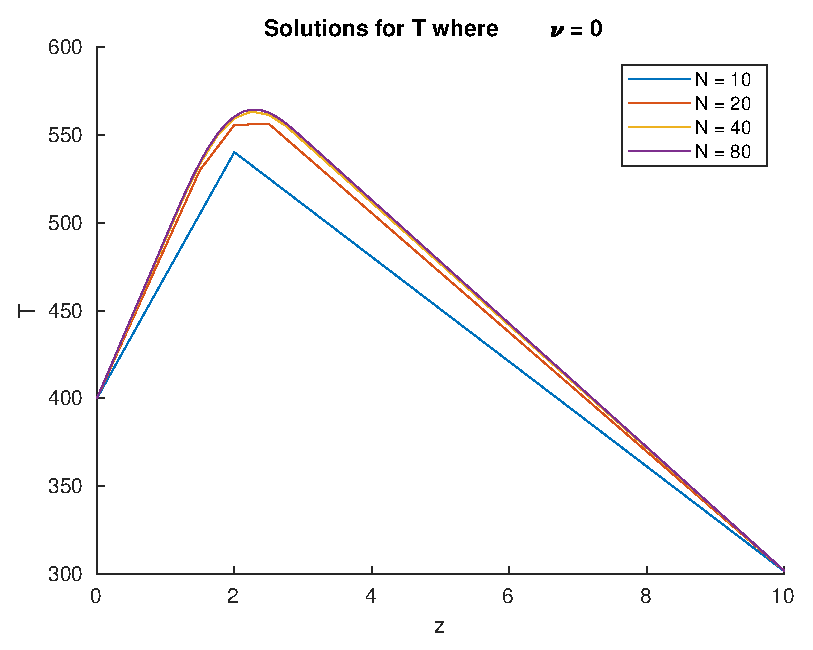
\includegraphics [width=4in]{lab1_01.eps}


\subsection*{Results - Diffusion \& Convection}

\begin{par}
Now we consider both diffusion and convection by taking nonzero $nu$. First we will look at $\nu = 0.1, 0.5, 1, 10$ for fixed $N = 40$.
\end{par} \vspace{1em}
\begin{par}
Upon inspection of the results, we see very crisp solutions for small $\nu$, but for $\nu = 10$ we have some artifacts of oscillations. Focussing first on $\nu = 0.1, 0.5, 1$, we see that as fluid velocity increases, the concentration of heat at the source diminishes. Instead, the fluid is able to absorb some heat and move that heat throughout the latter, unheated section of the tube.
\end{par} \vspace{1em}
\begin{par}
Focussing again on $\nu = 10$, we consider a few difference grid sizes, $N = 10, 20, 40$. The oscillations seem to have an amplitude that increases exponentially in $z$, but whose overall coefficient decreases as $N$ increases. One solution therefore would be to consider large N and only consider the solution on some subset [0,M] for M sufficiently smaller than L.
\end{par} \vspace{1em}
\begin{par}
Of course, if we have interest in the behavior of our solution near the right endpoint, we would have to consider altering our finite difference scheme to avoid the osillatory behavior. We can use the upwind method of replacing the first-order derivative's FD with a backward difference to circumvent the spurious oscillations for smaller h. We also plot numerical solutions using this method, and the improvement is obvious.
\end{par} \vspace{1em}
\begin{verbatim}
figure;   % New figure.
hold on;  % Allow for multiple plots on the same graph.
N = 40;   % Set number of grid intervals to 40.
for nu = [0.1 0.5 1 10]
    [Z, T] = lab1_solve(N, nu, @q);  % Run the solver.
    plot(Z, T, 'DisplayName', sprintf('\\nu = %.1f', nu));  % Plot.
end
xlabel('z');  % Label the axes.
ylabel('T');
legend;       % Enable the legend (defaults to DisplayName's).
title('Solutions for T with N = 40');  % Put a title.
snapnow;

figure;   % New figure.
hold on;  % Allow for multiple plots on the same graph.
nu = 10;  % Set fluid velocity to 10.
for N = 10*pow2(0:2)
    [Z, T] = lab1_solve(N, nu, @q);  % Run the solver.
    plot(Z, T, 'DisplayName', sprintf('N = %d', N));  % Plot the result.
end
xlabel('z');  % Label the axes.
ylabel('T');
legend;       % Enable the legend (defaults to DisplayName's).
title(sprintf('Solutions for T where \\nu = %d', nu));  % Put a title.
snapnow;

figure;  % New figure.
hold on;  % Allow for multiple plots on the same graph.
nu = 10;  % Set fluid velocity to 10.
for N = 10*pow2(0:2)
    [Z, T] = lab1_solve_upwind(N, nu, @q);  % Run the upwind solver.
    plot(Z, T, 'DisplayName', sprintf('N = %d', N));  % Plot the result.
end
xlabel('z');  % Label the axes.
ylabel('T');
legend;       % Enable the legend (defaults to DisplayName's).
title(sprintf('Upwind solutions for T where \\nu = %d', nu));  % Title.
snapnow;
\end{verbatim}

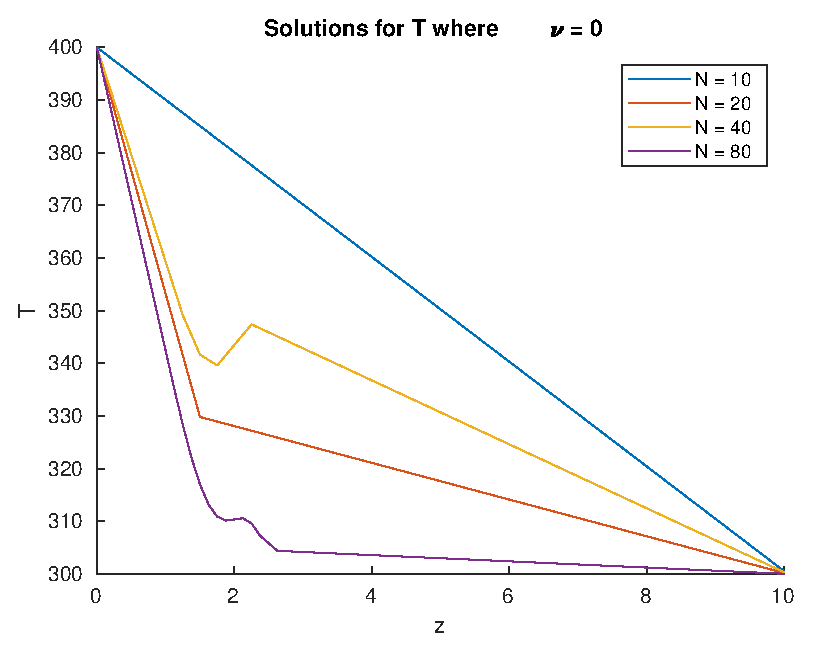
\includegraphics [width=4in]{lab1_02.eps}


\subsection*{Implementation of ODE solver}

\begin{par}
This section contains the implementation of the ODE solver.
\end{par} \vspace{1em}
\begin{verbatim}
function [Z, T] = lab1_solve(N, nu, q)
% LAB1_SOLVE: solves the linear ODE described in section `The Model and
%             Discretization` above.
%             Parameters:
%               N  - Number of segments to split the interval [0,L] into.
%               nu - Velocity of the fluid through the pipe.
%               q  - Forcing function s.t. D_T[T] = q(z).
%             Returns:
%               Z  - The N+1 values of [0,L] used in the dicretization.
%               T  - The N+1 approximate evaluations of T(Z).

global L kappa k rho C T_out T_0;

% Partition [0,L].
h = L/N;    % Width of our N intervals on [0,L].
Z = 0:h:L;  % Discrete support of our solution (excludes ghost points).

% Coefficients used in matrix A*.
D2_coeff = -kappa/h^2;            % Coefficient of T''(z).
D1_coeff = nu * rho * C / (2*h);  % Coefficient of T'(z).
% Value of constant K that comes up in the second boundary condition.
K = (2 * k / h) - (k * nu * rho * C / kappa);

% Linear coefficients of our derivative stencils.
% Here the vectors denote the coefficients along the tri-diagonals of the
% operators: [lower diagonal, major diagonal, upper diagonal].
D2 = [1 -2 1];  % Centered second order FD.
D1 = [-1 0 1];  % Centered first order FD.
DT = D2_coeff * D2 + D1_coeff * D1;  % Our differential operator D_T.

% Construction of matrix A*.
Cols = ones(N, 1) * DT;  % Columns of length N for the diagonals of A*.
% Construct A* as a sparse NxN matrix with the diagonals specified in Cols.
% -1:1 denotes the lower, major, and upper diagonals.
Astar = spdiags(Cols, -1:1, N, N);
% Account for BCs.
% Add K to matrix at the end of the major diagonal.
Astar(N, N) = Astar(N, N) + K;
% Add D2_coeff and D1_coeff to the end of the lower diagonal.
Astar(N, N-1) = Astar(N, N-1) + D2_coeff + D1_coeff;

% Construction of vector b*$.
bstar = q(Z(2:end)');  % Set b to the evaluation of Q on z_1, ..., z_N
% Account for the first boundary condition.
bstar(1) = bstar(1) + T_0 * (-D2_coeff + D1_coeff);
% Account for the second boundary condition.
bstar(end) = bstar(end) + K * T_out;

% Let T^0 be the solution of A* (.) = b*.
T_interior = Astar \ bstar;

% Add the approximations at the boundaries to T^0.
T = [T_0 ; T_interior ]';

end

function [Z, T] = lab1_solve_upwind(N, nu, q)
% LAB1_SOLVE_UPWIND: solves the linear ODE described in section `The Model
%                    and Discretization` above.
%                    Parameters:
%                      N  - Number of intervals on [0,L]
%                      nu - Velocity of the fluid through the pipe.
%                      q  - Forcing function s.t. D_T[T] = q(z).
%                    Returns:
%                      Z  - The N+1 values of [0,L] used.
%                      T  - The N+1 approximate evaluations of T(Z).

global L kappa k rho C T_out T_0;

% Partition [0,L].
h = L/N;    % Width of our N intervals on [0,L].
Z = 0:h:L;  % Discrete support of our solution.

% Coefficients used in matrix A_up
D2_coeff = -kappa/h^2;         % Coefficient of T''(z).
D1_coeff = nu * rho * C / h;   % Coefficient of T'(z).
% Value of constant K_up that comes up in the second boundary condition.
K_up = kappa / (h^2 * (kappa + k*h));

% Linear coefficients of our derivative stencils.
% Here the vectors denote the coefficients along the tri-diagonals of the
% operators: [lower diagonal, major diagonal, upper diagonal].
D2 = [1 -2 1];  % Centered second order FD.
D1 = [-1 1 0];  % Backward first order FD.
DT = D2_coeff * D2 + D1_coeff * D1;  % Our differential operator D_T.

% Construction of matrix A_up.
M = N-1;                 % Matrix dimension of A_up (in R^MxM).
Cols = ones(M, 1) * DT;  % Columns of length N for the diagonals of A_up.
% Construct A_up as a sparse MxM matrix w/ the diagonals specified in Cols.
% -1:1 denotes the lower, major, and upper diagonals.
Aup = spdiags(Cols, -1:1, M, M);
% Account for BCs.
% Remove K_up * kappa to matrix at the end of the major diagonal.
Aup(M, M) = Aup(M, M) - K_up*kappa;

% Construction of vector b*$.
bup = q(Z(2:end-1)');  % Set bup to the eval of Q on z_1, ..., z_{N-1}
% Account for the first boundary condition.
bup(1) = bup(1) + T_0 * (-D2_coeff + D1_coeff);
% Account for the second boundary condition.
bup(end) = bup(end) + K_up * k * h * T_out;

% Let T^0 be the solution of A* (.) = b*.
T_interior = Aup \ bup;

% Add the approximations at the boundaries to T^0.
t_N = (kappa*T_interior(end) + k*h*T_out)/(kappa + k*h);
T = [T_0 ; T_interior; t_N ]';
end

function Q = q(Z)
% Q: evaluates the driving heat function described in section `The Model
%    and Discretization` at each point in Z.
%    Parameters:
%      Z - points to evaluate the driving heat function at.
%    Returns:
%      Q - the evaluation of the heat function at each point in Z.

global a b Q_0;

% Logical index representing indices of Z that are inside the heating range
% of the coil.
heating_region = Z > a & Z < b;
% Values of Z in the heating region.
heated_zs = Z(heating_region);

% Create Q as a matrix where the only nonzero elements correspond
% to the values of Z that are in the heating_region.
Q = zeros(size(Z));
Q(heating_region) = Q_0 * sin(pi * (heated_zs - a) ./ (b - a));

end
\end{verbatim}

        \color{lightgray} \begin{verbatim}Infnorm for second-order linear soln w/ N=64 intervals: 7.389644e-13
Infnorm for second-order linear soln w/ N=128 intervals: 3.751666e-12
Infnorm for second-order linear soln w/ N=256 intervals: 9.720225e-12
Infnorm for second-order linear soln w/ N=512 intervals: 8.810730e-12
Infnorm for second-order linear soln w/ N=1024 intervals: 8.031975e-11
Estimated order of convergence for second-order linear soln:  1.761891

Infnorm for upwind linear soln w/ N=64 intervals: 1.818989e-11
Infnorm for upwind linear soln w/ N=128 intervals: 4.547474e-12
Infnorm for upwind linear soln w/ N=256 intervals: 2.649472e-10
Infnorm for upwind linear soln w/ N=512 intervals: 1.398348e-11
Infnorm for upwind linear soln w/ N=1024 intervals: 4.393655e-09
Estimated order of convergence for upwind linear soln:  5.100990

Infnorm for second-order sinusoidal soln w/ N=64 intervals: 2.106784e+00
Infnorm for second-order sinusoidal soln w/ N=128 intervals: 5.266210e-01
Infnorm for second-order sinusoidal soln w/ N=256 intervals: 1.316506e-01
Infnorm for second-order sinusoidal soln w/ N=512 intervals: 3.291235e-02
Infnorm for second-order sinusoidal soln w/ N=1024 intervals: 8.228097e-03
Estimated order of convergence for second-order sinusoidal soln:  2.000067

Infnorm for upwind sinusoidal soln w/ N=64 intervals: 2.456707e+02
Infnorm for upwind sinusoidal soln w/ N=128 intervals: 1.244540e+02
Infnorm for upwind sinusoidal soln w/ N=256 intervals: 6.263632e+01
Infnorm for upwind sinusoidal soln w/ N=512 intervals: 3.142116e+01
Infnorm for upwind sinusoidal soln w/ N=1024 intervals: 1.573654e+01
Estimated order of convergence for upwind sinusoidal soln:  0.991134

\end{verbatim} \color{black}
    
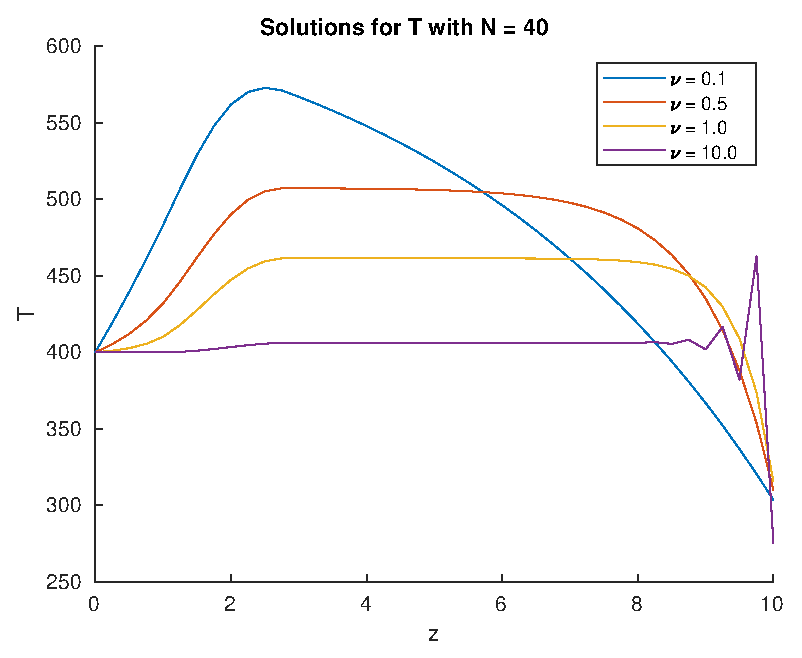
\includegraphics [width=4in]{lab1_03.eps}

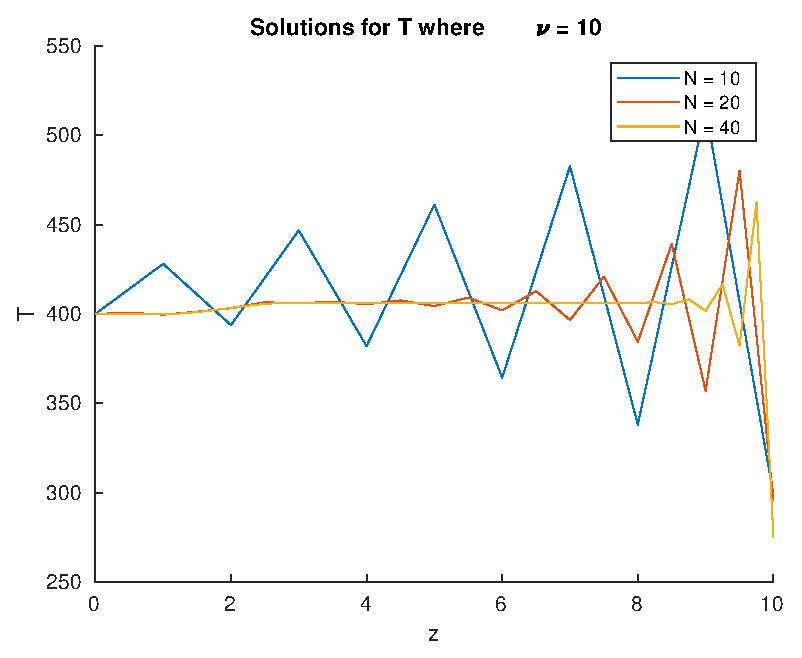
\includegraphics [width=4in]{lab1_04.eps}

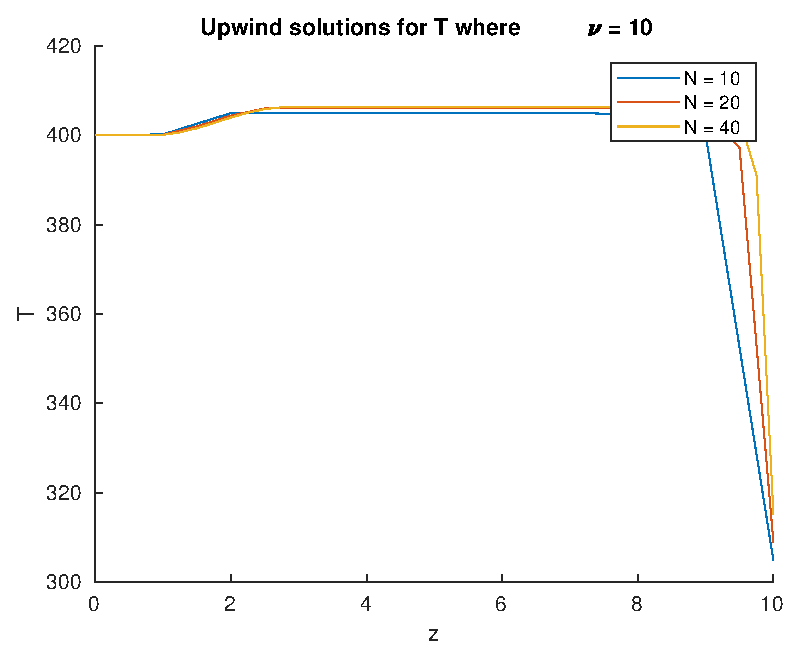
\includegraphics [width=4in]{lab1_05.eps}



\end{document}
    
